\chapter{Formación Inicial} \label{formacion}

% ********************************************************************

Para la elaboración de este trabajo ha sido necesario un período de formación en el que aprender acerca de distintas áreas específicas de la informática. El principal reto ha sido la aplicación de técnicas de inteligencia artificial, ya que la mención elegida durante la carrera fue Tecnologías de la Información, por tanto nunca había tratado con nada relacionado con modelos de \gls{IA}, \textit{clustering}, etc. Sin embargo, simplemente ha sido un reto más a superar. Para ello, se han llevado a cabo las siguientes actividades:

\subsubsection*{Curso Redes neurales y Aprendizaje profundo}

Este curso, impartido por Andrew Ng. et. al \cite{ng2023deep} y con una duración estimada de 4 semanas, proporcionaba las bases del funcionamiento de las \gls{RRNN} y el \gls{DL}. Cada semana debían visualizarse una serie de vídeos, realizar uno o varios cuestionarios e implementar un notebook para poner en práctica lo aprendido. Estaba formado por los siguientes módulos:

\begin{table}[H]
\centering
\footnotesize
\label{tab:course_modules}
\begin{tabularx}{\textwidth}{|c|X|c|c|c|}
\hline
\rowcolor{graylight}\texttt{Módulo} & \texttt{Descripción} & \texttt{Videos} & \texttt{Lecturas} & \texttt{Tareas} \\
\hline
1 & Análisis de las principales tendencias que impulsan el auge del aprendizaje profundo y ejemplos de dónde y cómo se aplica en la actualidad. & 6 & 3 & 1 \\
\hline
2 & Planteamiento de un problema de aprendizaje automático con una mentalidad de red neuronal y utilización de la vectorización para acelerar sus modelos. & 19 & 5 & 3 \\
\hline
3 & Construcción de una red neuronal con una capa oculta, utilizando la propagación hacia delante y la retropropagación. & 12 & 1 & 2 \\
\hline
4 & Análisis de los cálculos clave subyacentes al aprendizaje profundo y su utilización para construir y entrenar \gls{RRNN} profundas para tareas de \gls{VC}. & 8 & 7 & 3 \\
\hline
\end{tabularx}
\caption{Módulos del Curso de Deep Learning \& Neural Networks, Andrew Ng. \cite{ng2023deep}}
\end{table}

Finalmente, a pesar de no tener una relación tan estrecha con la implementación llevada a cabo en este proyecto, resultó de especial utilidad para entender conceptos básicos y poder hacer un uso consciente de la terminología, así como dar a conocer las principales librerías de Python utilizadas para el análisis de datos.

\vspace{1.5mm}

Fecha de finalización: 24 Octubre 2023

\vspace{-3.5mm}

\subsubsection*{Curso \gls{NLP} Hugging Face}

\vspace{-0.5mm}

Este segundo curso, aprendí los fundamentos del \gls{NLP}, qué son los encoders y los decoders, la librería de transformers y otra información de utilidad para el proyecto.

\begin{table}[H] 
\centering
\footnotesize
\label{tab:nlp_course_structure}
\begin{tabularx}{\textwidth}{|c|>{\hsize=.8\hsize}X|>{\hsize=1.2\hsize}X|}
\hline
\rowcolor{graylight}\texttt{Módulo} & \texttt{Sección} & \texttt{Contenido} \\
\hline
0 & Setup & Introduction \\
\hline
1 & Transformer models & Natural Language Processing; Transformers, what can they do?; How do Transformers work?; Encoder models; Decoder models
Sequence-to-sequence models; Bias and limitations \\
\hline
2 & Using transformers & Introduction; Behind the pipeline; Models; Tokenizers; Handling multiple sequences; Putting it all together; Basic usage completed! \\
\hline
3 & Fine-tuning a pretrained model & Introduction; Processing the data; Fine-tuning a model with the Trainer API or Keras; A full training; Fine-tuning, Check! \\
\hline
4 & Sharing models and tokenizers & Uploading model; Versions and models; Sharing across the ecosystem; DL and model card; Common concerns. \\
\hline
5 & The datasets library & Introduction; What if my dataset isn't on the Hub?; Time to slice and dice; Big data? Datasets to the rescue!; Creating your own dataset; Semantic search with FAISS; Datasets, check!  \\
\hline
6 & The tokenizers library & Introduction; Training a new tokenizer from an old one; Fast tokenizers' special powers; Fast tokenizers in the QA pipeline; Normalization and pre-tokenization; Byte-Pair Encoding tokenization; WordPiece tokenization; Unigram tokenization; Building a tokenizer, block by block; Tokenizers, check! \\
\hline
7 & Main NLP tasks & Introduction; Token classification; Fine-tuning a masked language model; Translation; Summarization; Training a causal language model from scratch; Question answering; Mastering NLP  \\
\hline
\end{tabularx}
\caption{Módulos del Curso de NLP de Hugging Face \cite{huggingface2023nlp}}
\end{table}

Fecha de finalización: 13 Enero 2024

\newpage

\subsubsection*{Resolución de módulos y máquinas de Capture The Flag}

Para aumentar mi formación en el ámbito de ciberseguridad, a lo largo de estos meses he llevado a cabo la resolución de las siguientes máquinas de \gls{CTF} y módulos en distintas plataformas:

\begin{table}[H]
\centering
\footnotesize
\label{tab:platform_solved_machines}
\begin{tabularx}{\textwidth}{|X|c|}
\hline
%\rowcolor[HTML]{4F81BD} 
\rowcolor{graylight}\texttt{Plataforma} & \texttt{Máquinas Resueltas} \\
\hline
TryHackMe & 109 \\
\hline
HackTheBox & 36 \\
\hline
Atenea & 1 \\
\hline
PortSwigger & 2 \\
\hline
\end{tabularx}
\caption{Máquinas de \textit{Hacking} Ético resueltas por Plataforma}
\end{table}

Entre estas máquinas, algunas me han resultado de especial interés, ya que me han proporcionado una base de conocimiento en relación a los Sistemas Operativos Linux y conceptos básicos de implementación de su seguridad:

\begin{figure}[H]
    \centering
    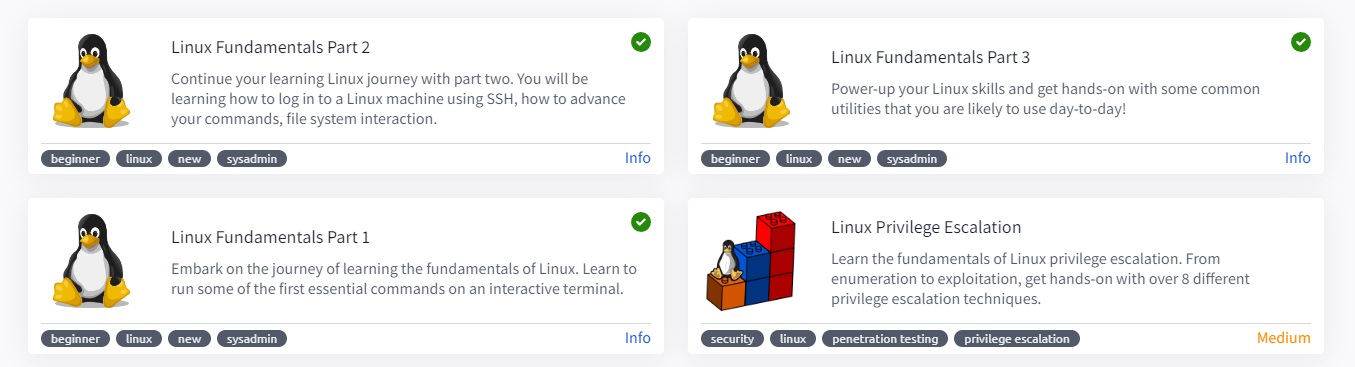
\includegraphics[width=1\linewidth]{imagenes/linux-thm.png}
    \caption{Módulos de TryHackMe sobre Fundamentos de Seguridad en Linux \cite{tryhackmelinux}}
    \label{fig:linux-thm}
\end{figure}

En ellos, se explican elementos como la gestión de permisos, el sistema de archivos de Linux, automatización o técnicas de \textit{hardening}. Otros módulos más específicos, como los que se muestran a continuación, ha resultado útiles para adquirir un mayor contexto acerca de los logs y su uso en sistemas de monitorización como los \gls{SIEM}:

\begin{figure}[H]
    \centering
    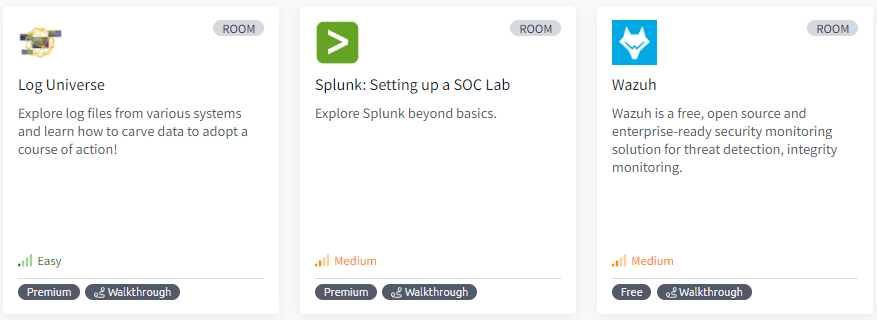
\includegraphics[width=1\linewidth]{imagenes/logs-thm1.png}
    \caption{Módulos de TryHackMe sobre Logs y Monitoreo de sistemas Linux I}
    \label{fig:logs-thm}
\end{figure}

\begin{figure}[H]
    \centering
    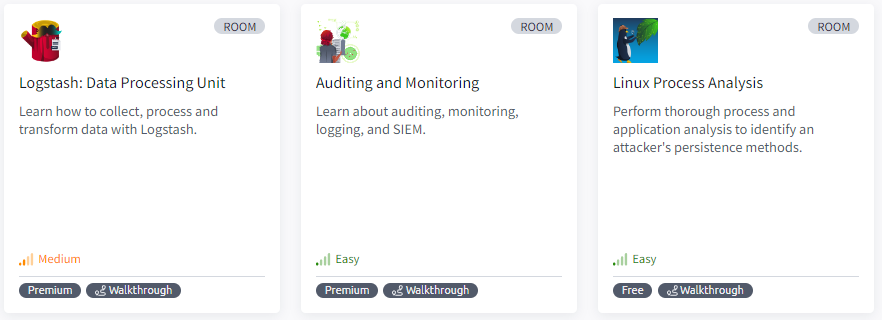
\includegraphics[width=1\linewidth]{imagenes/logs-thm2.png}
    \caption{Módulos de TryHackMe sobre Logs y Monitoreo de sistemas Linux II}
    \label{fig:logs-thm}
\end{figure}
